% Source ownership:
% - Arthur: conclusions


\section{Conclusions}
\label{sec:conclusions}

\subsection{Computer Simulation vs.\ Real-World Results}

While this Monte Carlo simulation successfully modelled the
conformational sampling of a polymer chain, it is important to
recognise the limitations when comparing theoretical calculations
to real-world experimental results.

\begin{itemize}
  \item By employing the OPLS-AA and TraPPE-UA force fields, we gain
    robust mathematical approximations of energy landscapes; however,
    these empirical potentials cannot fully capture the dynamic
    complexities of real-world solvent interactions or subtle quantum
    effects.
  \item The isolation of a single polymer chain within the simulation
    neglects the significant impact of intermolecular forces and
    environmental factors that would be present in a real-world
    scenario.
  \item The all-atom energy module applies a uniform backbone-position threshold
    to suppress short-range non-bonded interactions, which over-excludes some 1-5 and 1-6 hydrogen--hydrogen contacts. The impact is partially mitigated by the torsional potential and the single-chain, vacuum context of the simulation. Nonetheless, this represents a known approximation whose correction is left for future work.
\end{itemize}

\subsection{Nonlinearity of Parallel Speedup}

One of the key observations from our performance analysis is that
parallelisation rarely translates evenly into a 1:1 linear speedup.
In a perfect scenario, assigning four cores would make the code run
four times faster. However, as seen in our MPI benchmarks, adding
more workers inherently introduces communication overhead. The time
required for the orchestrator to pass messages, synchronise
coordinates during ensemble sampling, and track dynamic convergence
tests gradually eats into the raw processing speed. At certain
hardware boundaries, communication bottlenecks and competition for
physical system resources make additional core count benefits
negligible.

\subsection{Navigating Resource Utilization}

Combining multiple High-Performance Computing (HPC) methodologies --
such as MPI and OpenMP -- offers significant acceleration capabilities,
but requires careful resource management to prevent oversubscription.
Breaking up the simulation workflow into phases proved to be a critical
step in reusing resources and limiting the system size required to run
the program.

\subsection{HPC Optimization}

Ultimately, achieving high performance is not simply a matter of
checking whether a particular parallel processing technique outpaces
its serial counterpart; rather, it requires a coordinated benchmarking
strategy. Optimizing an HPC code ecosystem demands careful evaluation
of how different techniques overlap and complement one another. Were
this a commercial or funded research project, benchmarking the
performance of the various technique combinations (and against the
system hardware available) would be prudent.

Figure \ref{fig:scheme} illustrates our parallel processing architecture,
which leverages a central Master Node to efficiently orchestrate tasks
across the system. With combined optimization and parallelization
techniques, a possible workflow functions as follows:

\begin{itemize}
  \item The Master Node checks if an equilibrated geometry already
    exists, allowing it to bypass the computationally heavy equilibration
    phase for previously processed configurations (such as Conf 4, which
    immediately unlocks its production runs).
  \item For new configurations (like Confs 1 and 5), the system
    simultaneously deploys independent replicas.
  \item These replicas utilize a collaborative swarm logic, aided by
    the Geweke Convergence test running on 2 workers with 2 threads
    each, to dynamically find equilibrium as fast as possible.
  \item Since an equilibrated geometry for conformation type 4 is
    already supplied, the 2 workers with their 2 OpenMP threads each
    are immediately available to assist in the production runs for
    that configuration.
  \item Meanwhile equilibration completes for conformations 4 \& 5,
    and those workers become available to start assisting in the
    remaining jobs from the shared 30-job global production queue.
\end{itemize}

Total core count for this scenario (default when the parallel
submission script is invoked) is \textbf{13 cores}:

\begin{itemize}
  \item \textbf{1} Master Node (\textbf{1 core})
  \item 2 Workers each running a Conformation Equilibration
    \begin{itemize}
      \item Each of these workers takes 2 cores for Swarm Logic
        \begin{itemize}
          \item Each node calculates energy via 2 OpenMP threads
            ($2\times2\times2=$ \textbf{8 cores})
        \end{itemize}
    \end{itemize}
  \item 2 Workers immediately start production runs on
    equilibration-bypassed conformation~\#4. (\textit{Why 2? The
    system opts to utilize the same number of workers for a bypassed
    configuration as it would a swarm-logic equilibration.})
    \begin{itemize}
      \item These workers' energy calculations are threaded with
        OpenMP ($2\times2=$ \textbf{4 cores})
    \end{itemize}
  \item When the equilibration phase is done for conformations 1 \& 5,
    those workers are reassigned unfinished chunks of the production
    queue, \textit{reusing the CPU resources}, 4 cores per conformation.
    (\textbf{+0 cores})
  \item As workers finish their subtasks, they inform the orchestrator,
    receiving any pending jobs from the global queue until all 30
    production jobs are completed. (\textbf{+0 cores})
\end{itemize}

\begin{figure}[H]
  \centering
  
\includegraphics[width=0.8\textwidth]{ParallelProcessing_ResourceUtilization.png}
  \caption{Schematic view of the combined MPI/OpenMP resource utilization strategy.}
  \label{fig:scheme}
\end{figure}

\subsection{Wall Clock Comparison: Parallel vs Serial}

\begin{figure}[H]
  \centering
  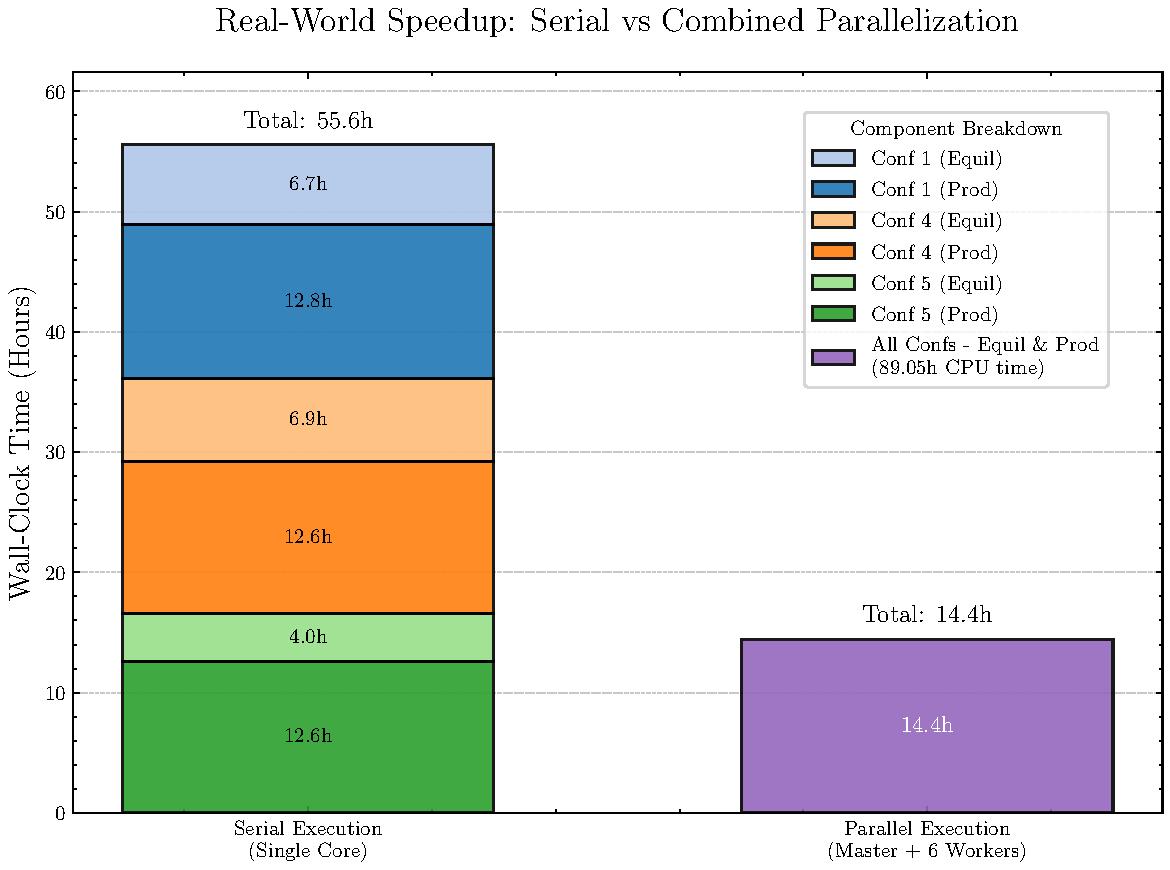
\includegraphics[width=0.8\textwidth]{figs/parallel_combined_v_serial_plot.pdf}
  \caption{Wall-Clock timing for serial vs combined parallelized simulation}
  \label{fig:par_v_ser}
\end{figure}

A final test of the parallelization efforts' efficiency was running the simulation serially, combining their runtimes, and comparing it to the wall-clock time required to complete the same parallel execution. No equilibration steps were bypassed to keep the comparison as similar as possible.

As seen in figure \ref{fig:par_v_ser}, the parallel version took 14h 26min to complete while the serial versions took a combined 55h 35m to perform the same tasks. The parallel version required 13 cores to operate, consisting of over 89h of compute time, not counting the master node's orchestration. The multi-processing approach condensed the parallel version's CPU-to-Wall clock time by a factor of \textbf{6.16x}, while the wall-to-wall clock speedup (parallel vs serial) was sped up by \textbf{3.85x}.

It's interesting to notice that while more resources are needed to run the parallel version, it was also able to complete all 3 configurations' equilibration and production simulations faster than the quickest serial simulation (Conf 5). This beautifully illustrates the contributions of high-performance computing architecture to scientific research, showing that it can assist in converting multi-day research bottlenecks into overnight jobs.